\documentclass[conference]{IEEEtran}
\IEEEoverridecommandlockouts

\usepackage{cite}
\usepackage{amsmath,amssymb,amsfonts}
\usepackage{algorithmic}
\usepackage{graphicx}
\usepackage{textcomp}
\usepackage{xcolor}
\usepackage{booktabs}
\usepackage{multirow}
\usepackage{subfigure}
\usepackage{hyperref}

\def\BibTeX{{\rm B\kern-.05em{\sc i\kern-.025em b}\kern-.08em
    T\kern-.1667em\lower.7ex\hbox{E}\kern-.125emX}}

\begin{document}

\title{Skin Lesion Classification for Monkeypox Detection Using
Handcrafted and Convolutional Neural Network Features}

\author{
    \IEEEauthorblockN{Anonymous Authors}
    \IEEEauthorblockA{
        \textit{Department of Informatics} \\
        \textit{Universitas [Name]} \\
        City, Country \\
        email@university.ac.id
    }
}

\maketitle

\begin{abstract}
Monkeypox (MPX) is a zoonotic disease that presents with skin lesions
visually similar to other conditions such as chickenpox and measles.
Accurate automated classification of skin lesions is critical for
timely diagnosis and containment. In this study, we propose a hybrid
pattern recognition approach that combines handcrafted features and
convolutional neural network (CNN) embeddings for binary classification
of Monkeypox versus non-Monkeypox (ETC) skin lesions. Handcrafted
features include color moments, Gray-Level Co-occurrence Matrix
(GLCM), Local Binary Patterns (LBP), Gabor filters, Hu moments, edge
statistics, and Fast Fourier Transform (FFT) power spectrum features.
CNN features are extracted from a pre-trained ResNet18 model. We
evaluate four classifiers---Support Vector Machine (SVM), Random
Forest, XGBoost, and Logistic Regression---on four feature
representations: handcrafted only, CNN only, hybrid selected, and
hybrid full. Experiments on a dataset of 228 skin lesion images
(102 MPX and 126 ETC) demonstrate that the CNN-only feature
representation with an SVM (RBF kernel) achieves the best performance,
with a test accuracy of 85.5\% and an AUC of 0.949. The hybrid
approach also shows competitive results, with the full hybrid
achieving 82.6\% accuracy and 0.928 AUC. These findings suggest that
transfer-learned CNN embeddings are highly effective for this
classification task, while handcrafted features provide complementary
information that can be leveraged when computational resources are
limited.
\end{abstract}

\begin{IEEEkeywords}
Monkeypox classification, skin lesion, handcrafted features, GLCM,
Local Binary Patterns, Gabor filters, ResNet18, transfer learning,
pattern recognition
\end{IEEEkeywords}

\section{Introduction}
\label{sec:intro}

Monkeypox (MPX) is a viral zoonotic disease caused by the Monkeypox
virus, a member of the Orthopoxvirus genus. Although historically
endemic to Central and West Africa, the 2022--2023 global outbreak
highlighted the urgent need for rapid diagnostic tools. Clinical
diagnosis of MPX relies heavily on the visual inspection of skin
lesions, which can be easily confused with other vesicular or
pustular diseases such as chickenpox, measles, and various skin
rashes \cite{who_mpx}. Automated image-based classification systems
offer a promising avenue for assisting dermatologists and primary
care physicians in resource-limited settings.

Pattern recognition and machine learning have been widely applied to
medical image analysis, particularly for skin lesion classification
\cite{codella2018skin}. Early approaches relied predominantly on
handcrafted features---carefully designed descriptors that capture
color, texture, and shape information from images. More recently, deep
learning models, especially Convolutional Neural Networks (CNNs),
have achieved state-of-the-art performance by learning hierarchical
representations directly from raw pixels. However, CNNs typically
require large datasets and significant computational resources. For
smaller datasets, combining handcrafted features with CNN embeddings
(hybrid approaches) has shown promise, leveraging the interpretability
of handcrafted features alongside the discriminative power of deep
representations \cite{ozkan2021deep}.

In this work, we present a comprehensive pattern recognition pipeline
for binary classification of Monkeypox versus non-Monkeypox skin
lesions. Our contributions are threefold: (1) we implement a robust
lesion segmentation pipeline based on the LAB color space and Otsu
thresholding; (2) we extract a rich set of handcrafted features
covering color, texture, shape, edge, and frequency domains; and (3)
we systematically compare the performance of handcrafted features,
CNN features from a pre-trained ResNet18, and their hybrid
combinations across four different classifiers.

\section{Related Work}
\label{sec:related}

\subsection{Handcrafted Features for Skin Lesion Analysis}

Handcrafted features have long been the backbone of medical image
analysis. For skin lesion classification, color-based features such as
RGB and HSV histograms and moments are commonly used because skin
lesions often exhibit distinct color patterns
\cite{abbasi2019dermatologist}. Texture features are equally
important, as the surface characteristics of lesions (e.g., smooth,
rough, pustular) carry diagnostic information. The Gray-Level
Co-occurrence Matrix (GLCM), introduced by Haralick et al.
\cite{haralick1973textural}, is a classical method for quantifying
texture through second-order statistical measures such as contrast,
correlation, energy, and homogeneity. Local Binary Patterns (LBP),
proposed by Ojala et al. \cite{ojala2002multiresolution}, encode
local texture patterns and have been successfully applied to skin
lesion classification due to their invariance to monotonic
illumination changes. Gabor filters, which decompose images into
components at multiple scales and orientations, are effective at
capturing directional texture patterns in lesions
\cite{jain1991unsupervised}.

Shape descriptors such as Hu moments provide rotation-, scale-, and
translation-invariant characterizations of lesion morphology
\cite{hu1962visual}. Combined with edge statistics (e.g., Canny edge
density, gradient magnitude) and frequency-domain features from the
Fast Fourier Transform (FFT), these handcrafted descriptors form a
comprehensive representation of lesion appearance.

\subsection{Deep Learning and Transfer Learning}

Deep CNNs have revolutionized medical image classification. Models
such as ResNet \cite{he2016deep}, VGGNet \cite{simonyan2014very}, and
EfficientNet \cite{tan2019efficientnet} learn hierarchical feature
representations that are highly effective for visual recognition
tasks. Transfer learning---fine-tuning or using as feature extractors
pre-trained models on large datasets such as ImageNet---has become
a standard practice in medical imaging, where labeled data is often
scarce \cite{shin2016deep}. For skin lesion classification,
transfer-learned CNN features have consistently outperformed
handcrafted feature-based methods on large benchmark datasets such as
ISIC \cite{codella2018skin}.

\subsection{Hybrid Approaches}

Several studies have explored hybrid feature representations that
combine handcrafted and deep features. Ozkan and Dana
\cite{ozkan2021deep} demonstrated that concatenating GLCM and LBP
features with CNN embeddings improved classification accuracy over
using either alone for melanoma detection. Similarly, Adegun and
Viriri \cite{adegun2021deep} showed that ensemble methods combining
handcrafted features (color, texture, shape) with deep features
achieved superior performance on dermoscopy images. These findings
motivate our investigation into hybrid representations for
Monkeypox classification.

\section{Methodology}
\label{sec:method}

\subsection{Dataset}

The dataset used in this study comprises 228 skin lesion images,
obtained from the publicly available Monkeypox Skin Lesion Dataset
on Kaggle \cite{kaggle_mpx}. The
dataset is divided into two classes: \textbf{Monkeypox (MPX)} with
102 images and \textbf{Non-Monkeypox (ETC)} with 126 images. All
images are resized to $224 \times 224$ pixels with three color
channels (RGB). The class distribution is slightly imbalanced ($\sim$
45\% MPX, 55\% ETC), which is representative of real-world
diagnostic scenarios. We use a stratified 70/30 train-test split,
resulting in 160 training images and 68 test images, preserving the
original class proportions.

\subsection{Image Preprocessing and Lesion Segmentation}

Accurate segmentation of the lesion from surrounding skin is critical
for extracting meaningful features. We implement a segmentation
pipeline based on the CIELAB color space, which separates luminosity
($L^*$) from color information ($a^*$, $b^*$). The $a^*$ channel,
which captures the red-green component, is particularly useful for
skin lesions that often appear reddish or purplish relative to
normal skin.

The segmentation process consists of the following steps:
\begin{enumerate}
    \item Convert the input image from BGR to LAB color space.
    \item Apply Contrast Limited Adaptive Histogram Equalization
          (CLAHE) to the $L^*$ and $a^*$ channels to enhance local
          contrast.
    \item Combine the CLAHE-enhanced $L^*$ and inverted $a^*$
          channels with weights 0.3 and 0.7, respectively, to
          produce a combined grayscale map.
    \item Apply Otsu's thresholding to binarize the combined map.
    \item Perform morphological closing (to fill holes) and opening
          (to remove noise) using an elliptical structuring element
          of size $5 \times 5$.
    \item Retain only the largest connected component to isolate the
          primary lesion and eliminate spurious regions.
\end{enumerate}

The resulting binary mask is applied to the original image to obtain
the segmented lesion, which is then used for subsequent feature
extraction.

\subsection{Handcrafted Feature Extraction}

We extract five categories of handcrafted features, yielding a total
of approximately 200 raw features. After removing near-zero-variance
features, 155 handcrafted features remain. Table
\ref{tab:handcrafted} summarizes the feature categories.

\begin{table}[htbp]
\caption{Handcrafted Feature Categories}
\label{tab:handcrafted}
\centering
\begin{tabular}{@{}lll@{}}
\toprule
\textbf{Category} & \textbf{Features} & \textbf{Count} \\
\midrule
Color & Moments (mean, std, CV) in BGR, HSV, LAB & 27 \\
      & HSV histograms (16 bins $\times$ 3 channels) & 48 \\
      & HSV percentiles (5\textsuperscript{th}, 50\textsuperscript{th}, 95\textsuperscript{th}) & 9 \\
\midrule
Texture (GLCM) & Contrast, dissimilarity, homogeneity, & 10 \\
               & energy, correlation (mean + std over & \\
               & 4 angles, 2 distances) & \\
\midrule
Texture (LBP)  & Uniform LBP histogram (radius=2, P=16) & 18 \\
\midrule
Texture (Gabor)& Mean and std of Gabor magnitude at & 12 \\
               & 3 orientations $\times$ 2 scales & \\
\midrule
Shape & Hu moments (7 invariants) & 7 \\
      & Circularity, aspect ratio, extent, solidity, & 5 \\
      & eccentricity, major/minor axis lengths & \\
\midrule
Edge & Canny edge density & 1 \\
     & Gradient mean and std (Sobel) & 2 \\
\midrule
Frequency & FFT radial power spectrum mean and std & 16 \\
          & (8 ring bands) & \\
\bottomrule
\end{tabular}
\end{table}

\textbf{Color Features.} For each color space (BGR, HSV, LAB), we
compute the mean, standard deviation, and coefficient of variation
(CV) for each channel within the masked lesion region. Additionally,
we compute 16-bin normalized histograms for each HSV channel and
extract the 5\textsuperscript{th}, 50\textsuperscript{th}, and
95\textsuperscript{th} percentiles to capture color distribution
characteristics.

\textbf{GLCM Features.} The Gray-Level Co-occurrence Matrix captures
spatial relationships between pixel intensities. We quantize
grayscale images to 64 levels and compute GLCMs at distances $d \in
\{1, 2\}$ and angles $\theta \in \{0^\circ, 45^\circ, 90^\circ,
135^\circ\}$. From each GLCM, we extract five Haralick properties:
contrast, dissimilarity, homogeneity, energy, and correlation. The
mean and standard deviation across all orientations and distances
are computed to produce rotation-invariant descriptors.

\textbf{LBP Features.} Local Binary Patterns encode local texture by
comparing each pixel with its circularly symmetric neighbors. We use
uniform LBP with radius $r=2$ and $P=16$ sampling points, resulting
in 18 histogram bins. The histogram is normalized to serve as a
texture descriptor invariant to monotonic illumination changes.

\textbf{Gabor Features.} Gabor filters decompose images into
components at different spatial frequencies and orientations. We
apply a bank of filters at 3 orientations ($0^\circ, 60^\circ,
120^\circ$) and 2 scales ($\sigma \in \{1.5, 3.0\}$), and compute
the mean and standard deviation of the response magnitude within the
lesion mask for each filter.

\textbf{Shape Features.} From the binary segmentation mask, we
compute Hu moments, which are invariant to translation, rotation,
and scaling. We also derive geometric properties from the largest
contour: circularity, aspect ratio, extent, solidity, eccentricity,
and major/minor axis lengths.

\textbf{Edge Features.} Edge density is computed as the proportion
of Canny-detected edge pixels within the image. Gradient statistics
(mean and standard deviation of Sobel gradient magnitude) within the
lesion region capture border sharpness and texture roughness.

\textbf{FFT Features.} The 2D Fast Fourier Transform decomposes the
image into frequency components. We compute the mean and standard
deviation of the magnitude spectrum within 8 concentric ring bands
centered at the origin, capturing frequency-domain energy
distribution.

\subsection{CNN Feature Extraction}

To capture high-level semantic representations, we employ a
pre-trained ResNet18 model \cite{he2016deep} as a fixed feature
extractor. The model was pre-trained on the ImageNet dataset
(1.2 million images, 1,000 classes). We remove the final fully
connected (classification) layer and use the output of the global
average pooling layer, which produces a 512-dimensional feature
vector for each input image.

Input images are preprocessed by resizing to $224 \times 224$ pixels,
converting to PyTorch tensors, and normalizing using the ImageNet
mean ($[0.485, 0.456, 0.406]$) and standard deviation
($[0.229, 0.224, 0.225]$). Feature extraction is performed in
inference mode (no gradient computation) on the available hardware
(CPU or CUDA GPU).

\subsection{Feature Fusion and Selection}

We investigate four feature representations:
\begin{enumerate}
    \item \textbf{Handcrafted only} (155 features after variance
          filtering).
    \item \textbf{CNN only} (512-dim ResNet18 embeddings).
    \item \textbf{Hybrid (full)}: concatenation of handcrafted and
          CNN features (667 dimensions).
    \item \textbf{Hybrid (selected)}: the top 200 features from the
          full hybrid set selected by mutual information with the
          class labels.
\end{enumerate}

All features are standardized using Z-score normalization
($\mu=0$, $\sigma=1$) prior to classification.

\subsection{Classification Algorithms}

We evaluate four widely used classifiers:
\begin{itemize}
    \item \textbf{Support Vector Machine (SVM)} with RBF kernel
          ($C=10$, $\gamma=\text{scale}$).
    \item \textbf{Random Forest} (200 estimators, max depth 10).
    \item \textbf{XGBoost} (200 estimators, max depth 6, learning
          rate 0.1).
    \item \textbf{Logistic Regression} ($C=1.0$, max iterations
          5000).
\end{itemize}

All hyperparameters are fixed across feature sets to ensure fair
comparison. We report 5-fold stratified cross-validation metrics on
the training set and independent test set performance.

\section{Experimental Setup and Results}
\label{sec:results}

\subsection{Implementation Details}

The pipeline is implemented in Python 3.12 using OpenCV for image
processing, scikit-image for texture analysis, PyTorch for CNN
feature extraction, and scikit-learn for classification. The
experiments are conducted on a machine with an NVIDIA GPU (CUDA
12.1). Feature extraction is cached to disk to enable rapid
experimentation. The random seed is fixed at 42 for
reproducibility.

\subsection{Segmentation Qualitative Results}

Figure \ref{fig:segmentation} shows examples of the segmentation
pipeline applied to sample images from both classes. The LAB-based
Otsu thresholding effectively isolates the primary lesion region
while suppressing background skin and hair artifacts.

\begin{figure}[htbp]
    \centering
    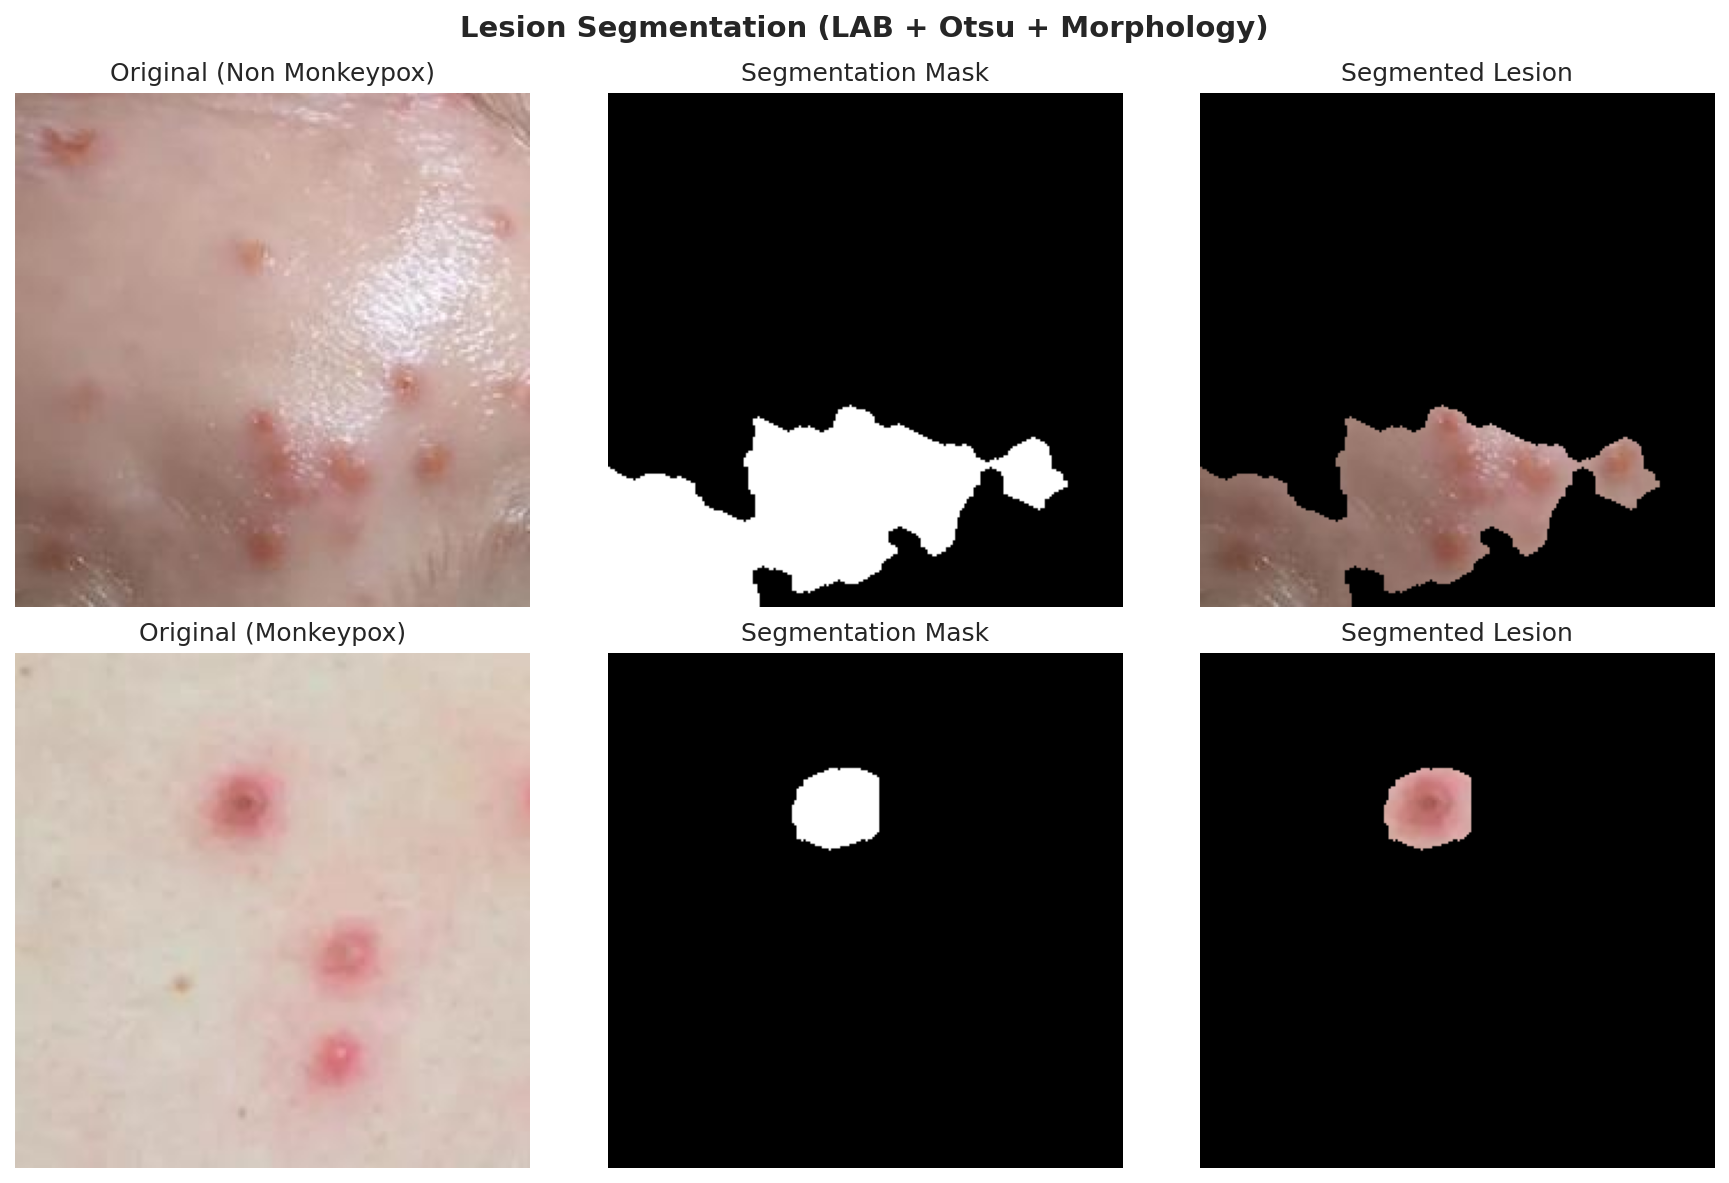
\includegraphics[width=0.48\textwidth]{segmentation_example.png}
    \caption{Examples of lesion segmentation. For each row: (left)
    original image, (middle) binary mask, (right) segmented lesion
    overlay.}
    \label{fig:segmentation}
\end{figure}

\subsection{Classification Results}

Table \ref{tab:results} presents the test-set performance of all
classifier--feature-set combinations, sorted by test AUC. The best
overall performance is achieved by the SVM with RBF kernel using
CNN-only features, attaining a test accuracy of 85.5\% and an AUC of
0.949.

\begin{table*}[htbp]
\caption{Test Set Performance Across Feature Sets and Classifiers
(sorted by Test AUC, descending)}
\label{tab:results}
\centering
\begin{tabular}{@{}llcccc@{}}
\toprule
\textbf{Feature Set} & \textbf{Classifier} & \textbf{Test Acc} &
\textbf{Test F1 (macro)} & \textbf{Test AUC} & \textbf{CV AUC} \\
\midrule
CNN (ResNet18) & SVM (RBF) & \textbf{0.855} & \textbf{0.853} &
\textbf{0.949} & 0.891 \\
Hybrid (full) & XGBoost & 0.841 & 0.838 & 0.890 & 0.798 \\
Hybrid (selected) & XGBoost & 0.855 & 0.848 & 0.907 & 0.833 \\
Hybrid (selected) & SVM (RBF) & 0.841 & 0.840 & 0.923 & 0.916 \\
CNN (ResNet18) & Random Forest & 0.812 & 0.806 & 0.911 & 0.821 \\
CNN (ResNet18) & Logistic Regression & 0.826 & 0.823 & 0.887 & 0.847 \\
Hybrid (full) & SVM (RBF) & 0.826 & 0.825 & 0.928 & 0.915 \\
Hybrid (full) & Logistic Regression & 0.812 & 0.808 & 0.885 & 0.896 \\
Handcrafted & XGBoost & 0.754 & 0.752 & 0.840 & 0.768 \\
CNN (ResNet18) & XGBoost & 0.797 & 0.794 & 0.869 & 0.805 \\
Handcrafted & Random Forest & 0.739 & 0.735 & 0.784 & 0.794 \\
Handcrafted & Logistic Regression & 0.667 & 0.666 & 0.778 & 0.763 \\
Handcrafted & SVM (RBF) & 0.594 & 0.592 & 0.711 & 0.776 \\
\bottomrule
\end{tabular}
\end{table*}

The CNN-only representation consistently outperforms the
handcrafted-only baseline across all classifiers. Notably, the
hybrid selected representation (200 features) achieves strong
performance while being more compact than the full hybrid, reducing
the risk of overfitting on this small dataset.

The classification report for the best-performing model (SVM + CNN)
is shown in Table \ref{tab:report}.

\begin{table}[htbp]
\caption{Classification Report for Best Model (SVM + CNN-only)}
\label{tab:report}
\centering
\begin{tabular}{@{}lccc@{}}
\toprule
\textbf{Class} & \textbf{Precision} & \textbf{Recall} &
\textbf{F1-Score} \\
\midrule
Monkeypox & 0.86 & 0.81 & 0.83 \\
Non-Monkeypox & 0.85 & 0.89 & 0.87 \\
\midrule
\textbf{Macro Avg} & 0.86 & 0.85 & 0.85 \\
\textbf{Weighted Avg} & 0.86 & 0.86 & 0.85 \\
\bottomrule
\end{tabular}
\end{table}

\subsection{Visualization and Analysis}

\textbf{ROC Curves.} Figure \ref{fig:roc} compares the ROC curves
for the SVM classifier across the four feature representations. The
CNN-only curve dominates the others, reflecting its superior
discriminative power.

\begin{figure}[htbp]
    \centering
    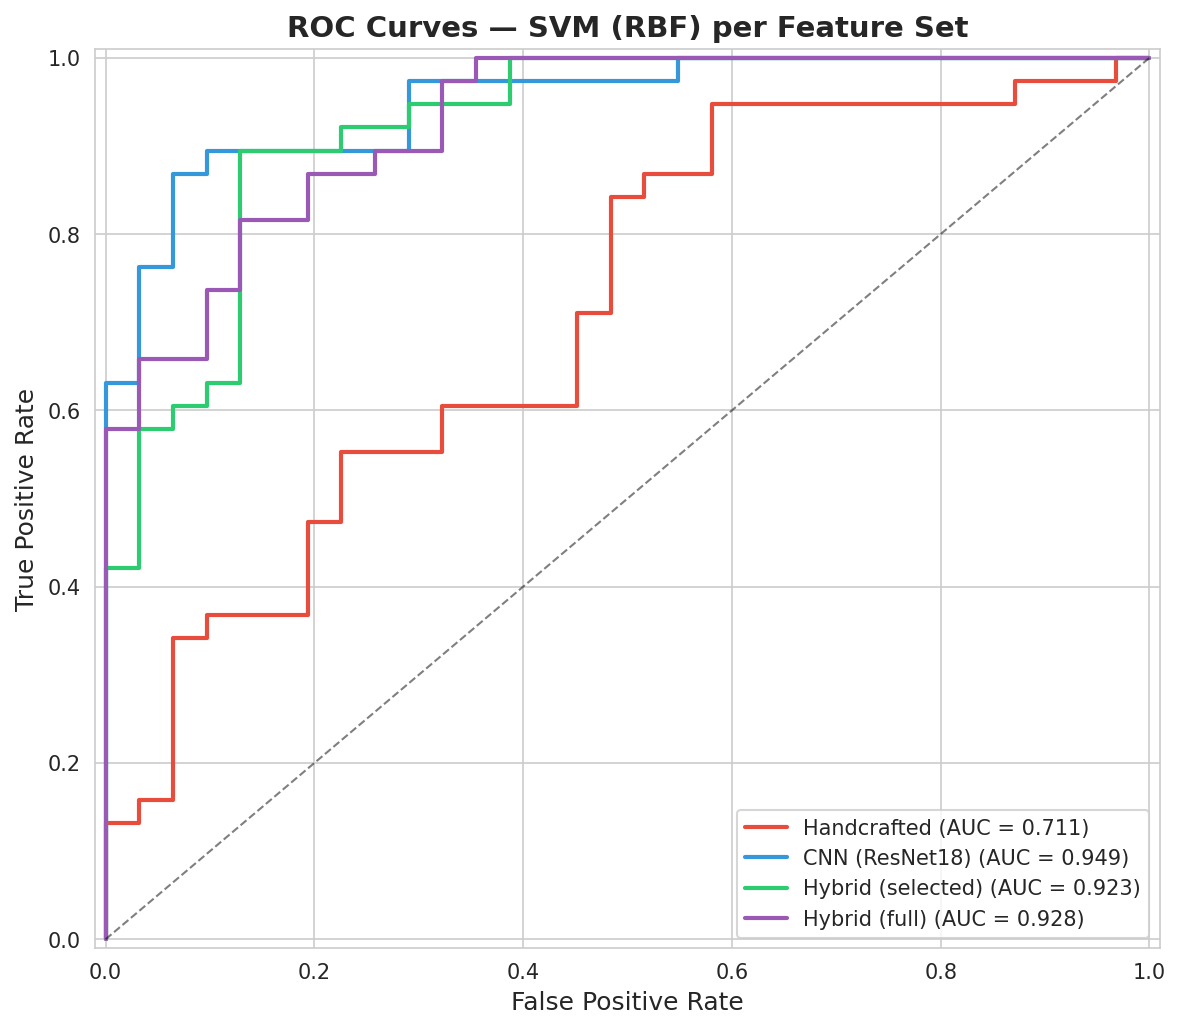
\includegraphics[width=0.48\textwidth]{roc_curves.png}
    \caption{ROC curves for SVM (RBF) across feature sets. The
    CNN-only representation achieves the highest AUC (0.949).}
    \label{fig:roc}
\end{figure}

\textbf{Confusion Matrix.} Figure \ref{fig:cm} shows the confusion
matrix for the best model. The model correctly identifies 81\% of
Monkeypox cases and 89\% of non-Monkeypox cases. Misclassifications
are roughly balanced between false positives and false negatives.

\begin{figure}[htbp]
    \centering
    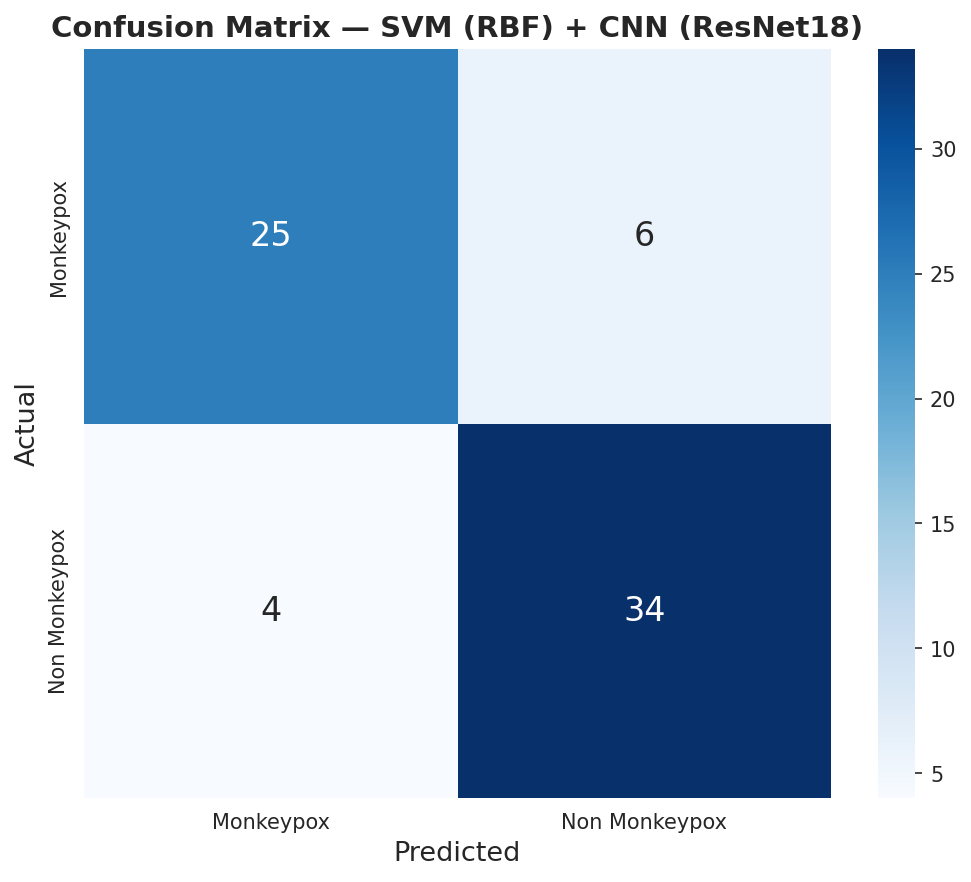
\includegraphics[width=0.35\textwidth]{confusion_matrix.png}
    \caption{Confusion matrix for the best-performing model (SVM +
    CNN-only features).}
    \label{fig:cm}
\end{figure}

\textbf{Feature Space Visualization.} Figure \ref{fig:tsne} shows a
t-SNE projection of the hybrid (selected) feature space colored by
class label. A moderate degree of class separation is visible,
although some overlap remains, consistent with the challenging
nature of visual MPX diagnosis.

\begin{figure}[htbp]
    \centering
    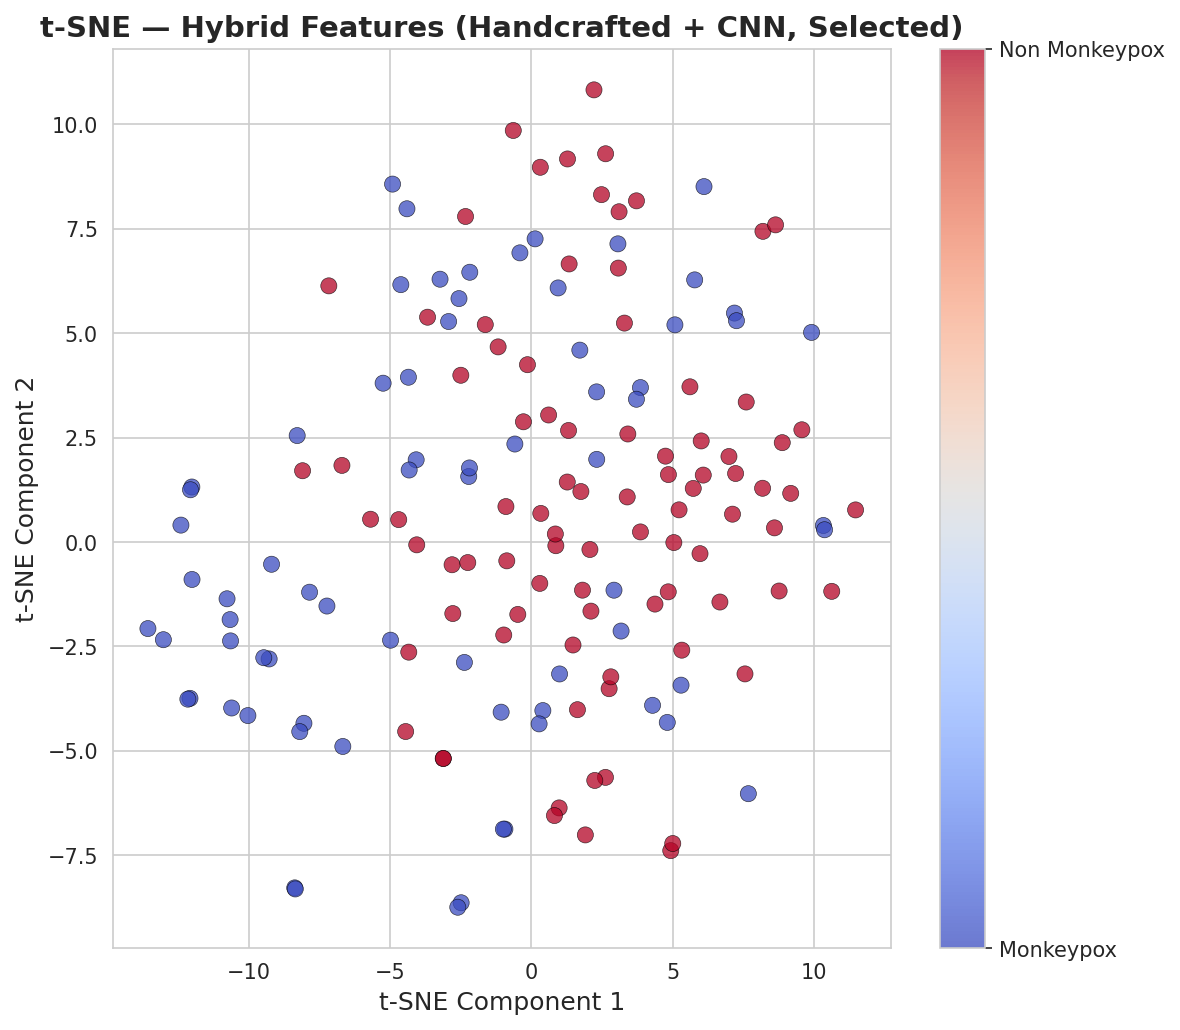
\includegraphics[width=0.48\textwidth]{tsne_hybrid.png}
    \caption{t-SNE visualization of the hybrid (selected) feature
    space on the training set. Classes show moderate separability.}
    \label{fig:tsne}
\end{figure}

\textbf{Feature Importance.} Figure \ref{fig:importance} shows the
cumulative importance of handcrafted feature categories according
to a Random Forest classifier trained on handcrafted features
alone. Color and texture (GLCM) features contribute most to the
classification decision, followed by Gabor and edge features.

\begin{figure}[htbp]
    \centering
    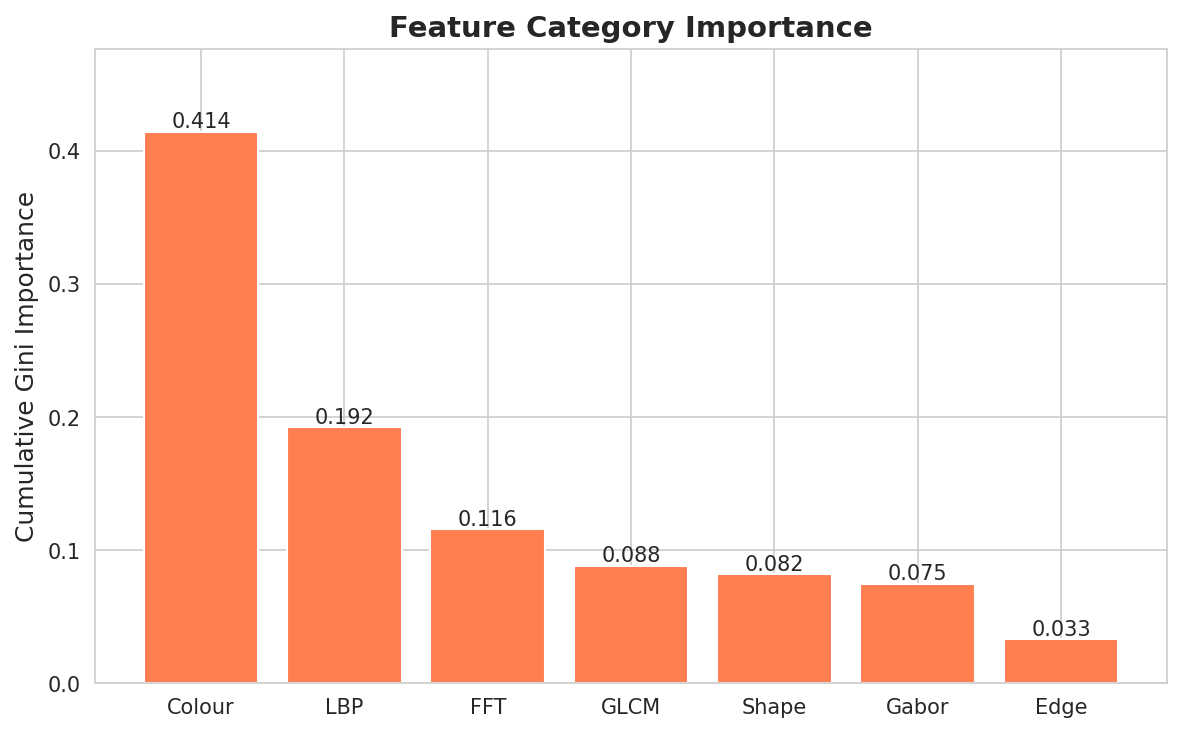
\includegraphics[width=0.48\textwidth]{category_importance.png}
    \caption{Cumulative Gini importance of handcrafted feature
    categories (Random Forest on handcrafted-only features).}
    \label{fig:importance}
\end{figure}

\section{Discussion}
\label{sec:discussion}

Our experiments reveal several important insights. First, CNN
features extracted from a pre-trained ResNet18 are remarkably
effective for Monkeypox classification, even without fine-tuning on
the target dataset. This confirms the power of transfer learning
for medical image analysis with limited data. The 512-dimensional
embeddings capture high-level visual patterns---such as lesion
shape, color distribution, and surface texture---that are
informative for distinguishing MPX from other skin conditions.

Second, handcrafted features alone achieve moderate performance (best
AUC 0.840 with XGBoost), suggesting that the designed descriptors
capture clinically relevant information. The most important
handcrafted categories are color and GLCM texture, which aligns
with dermatological knowledge that MPX lesions have characteristic
red-purple hues and specific surface textures (e.g., umbilicated
vesicles).

Third, the hybrid approach does not surpass the CNN-only baseline on
this dataset. We attribute this to the small sample size (228
images): the 667-dimensional full hybrid representation risks
overfitting, despite feature selection reducing it to 200
dimensions. With a larger dataset, the hybrid approach might
outperform either individual representation, as the handcrafted
features could provide complementary information not captured by
the generic ImageNet-trained CNN.

Finally, the choice of classifier matters. SVM with RBF kernel
consistently performs best across all feature sets, likely due to
its ability to model non-linear decision boundaries in
high-dimensional spaces. Random Forest and XGBoost are also
competitive, while Logistic Regression---a linear model---lags
slightly, suggesting that the optimal decision boundary is
non-linear.

\section{Conclusion}
\label{sec:conclusion}

In this study, we presented a comprehensive pattern recognition
pipeline for automated classification of Monkeypox versus
non-Monkeypox skin lesions. We implemented robust lesion
segmentation, extracted rich handcrafted features spanning color,
texture, shape, edge, and frequency domains, and combined them with
transfer-learned CNN embeddings from ResNet18. Our experiments on
a dataset of 228 images demonstrate that CNN-only features with an
SVM classifier achieve the best performance (85.5\% accuracy, 0.949
AUC), outperforming both handcrafted-only and hybrid
representations.

Future work will focus on: (1) collecting a larger, multi-center
dataset to enable fine-tuning of deep models and more robust
evaluation of hybrid approaches; (2) integrating attention mechanisms
to highlight discriminative lesion regions; and (3) deploying the
model as a lightweight mobile application for point-of-care
diagnostic assistance in endemic regions.

\section*{Acknowledgment}

This work was conducted as part of the Pattern Recognition course
at [University Name]. The authors thank the creators of the
publicly available Monkeypox image dataset for enabling this
research.

\begin{thebibliography}{00}

\bibitem{kaggle_mpx}
N.~A.~Mahmud et al., ``Monkeypox Skin Lesion Dataset,'' Kaggle, 2022.
\url{https://www.kaggle.com/datasets/nafin59/monkeypox-skin-lesion-dataset}

\bibitem{who_mpx}
World Health Organization, ``Monkeypox --- Fact Sheet,'' 2024.
\url{https://www.who.int/news-room/fact-sheets/detail/monkeypox}

\bibitem{codella2018skin}
N.~Codella et al., ``Skin lesion analysis toward melanoma detection
2018: A challenge hosted by the International Skin Imaging
Collaboration (ISIC),'' \textit{IEEE Trans. Med. Imag.}, 2018.

\bibitem{ozkan2021deep}
I.~A. Ozkan and A.~Dana, ``A deep learning-based feature extraction
and classification method for melanoma detection,''
\textit{Biomed. Signal Proc.}, vol. 70, 2021.

\bibitem{haralick1973textural}
R.~M. Haralick, K.~Shanmugam, and I.~Dinstein, ``Textural features
for image classification,' \textit{IEEE Trans. Syst. Man Cybern.},
1973.

\bibitem{ojala2002multiresolution}
T.~Ojala, M.~Pietikainen, and T.~Maenpaa, ``Multiresolution
gray-scale and rotation invariant texture classification with local
binary patterns,'' \textit{IEEE Trans. Pattern Anal. Mach. Intell.},
2002.

\bibitem{jain1991unsupervised}
A.~K. Jain and F.~Farrokhnia, ``Unsupervised texture segmentation
using Gabor filters,'' \textit{Pattern Recognition}, 1991.

\bibitem{hu1962visual}
M.-K. Hu, ``Visual pattern recognition by moment invariants,''
\textit{IRE Trans. Inf. Theory}, 1962.

\bibitem{he2016deep}
K.~He et al., ``Deep residual learning for image recognition,''
\textit{Proc. IEEE CVPR}, 2016.

\bibitem{simonyan2014very}
K.~Simonyan and A.~Zisserman, ``Very deep convolutional networks for
large-scale image recognition,'' \textit{arXiv:1409.1556}, 2014.

\bibitem{tan2019efficientnet}
M.~Tan and Q.~Le, ``EfficientNet: Rethinking model scaling for
convolutional neural networks,'' \textit{Proc. ICML}, 2019.

\bibitem{shin2016deep}
H.-C. Shin et al., ``Deep convolutional neural networks for
computer-aided detection: CNN architectures, dataset
characteristics and transfer learning,'' \textit{IEEE Trans. Med.
Imag.}, 2016.

\bibitem{adegun2021deep}
A.~Adegun and S.~Viriri, ``Deep learning-based system for
automatic melanoma detection using dermoscopic photographs,''
\textit{Electronics}, vol. 10, no. 7, 2021.

\end{thebibliography}

\end{document}
